\chapter{Discussion}\label{Discussion}

The main motivation for this work was the observation that characteristic sparse representations tend to emerge from sparse coding models trained over a variety of natural scene datasets by a variety of learning algorithms. The theorems proven here provide some insight into this phenomenon by establishing very general conditions under which identification of the model parameters is not only possible but also robust to measurement and modeling error.

The guarantees concerning the identification of a dictionary and corresponding sparse codes of minimal average support size (Thm.~\ref{SLCopt}), which is the optimization problem of most interest to practitioners (Prob.~\ref{OptimizationProblem}), are to my knowledge the first of their kind in both the noise-free and noisy domains. It has been shown here that, given sufficient data, this problem reduces to an instance of Prob.~\ref{InverseProblem} to which the main result (Thm.~\ref{DeterministicUniquenessTheorem}) then applies: every dictionary and corresponding set of sparse codes consistent with the data are equivalent up to inherent relabeling/scaling ambiguities and a discrepancy (error) that scales linearly with the noise. 
In fact, %provided $n \geq \min(2k,m)$, 
in almost all cases these problems are well-posed given a sufficient amount of data (Thm.~\ref{robustPolythm} and Cor.~\ref{ProbabilisticCor}). 
Furthermore, the derived scaling constants are explicit and computable; as such, there is an effective procedure that suffices to affirm if a proposed solution to these problems is indeed unique up to noise and inherent ambiguities, although it is not efficient in general. %Specifically, given a dictionary and sparse codes purported to solve to Prob.~\ref{InverseProblem}, one checks that that they satisfy the corresponding constraints on $\mathbf{A}$ and the $\mathbf{x_i}$ given in the statement of Thm.~\ref{DeterministicUniquenessTheorem}. 

%to the recovery of ``mouse neuronal activity representing location on a track \cite{agarwal2014spatially}

%Beyond an extension of existing noiseless guarantees \cite{Hillar15} to the noisy regime and their novel application to Prob.~\ref{OptimizationProblem}, this work contains a theory of combinatorial designs for support sets key to identification of dictionaries. This idea is incorporated into a fundamental lemma in matrix theory (Lem.~\ref{MainLemma}) that draws upon the definition of a matrix lower bound (\ref{Ldef}) induced by a hypergraph. As a consequence of this combinatorial approach, recovery of some or all dictionary elements can be guaranteed even if: i) dictionary size is overestimated, ii) data cover only a polynomial number of distinct sparse supports, and iii) dictionaries do not satisfy the spark condition. 

While the extension from exact recovery to the noisy stability of dictionary learning may be significant, the fact that the analysis relies on metrics of the data that are not feasible to compute limits its impact to the scientific community beyond computer science and applied mathematics. Consequently, the inferences of those applying dictionary learning methods to inverse problems in their research are justified only in principle; but this is unavoidably the case for NP-hard problems. What sets the main results of this work apart from the vast majority of results in the field, however, is their deterministic nature. They do not depend on any kind of assumption about the particular random distribution from which the sparse supports, coefficients, or dictionary entries are drawn (e.g., Cor.~\ref{ProbabilisticCor} makes a sweeping statement applicable to all continuous distributions). 

Indeed, theoretical validation makes little practical difference if the methodology is already in widespread use, while practical criteria establishing whether the data models obtained by practitioners are optimal or not would have very high impact. To this end, the work has been laid out for those wanting to derive statistical criteria for inference with respect to more domain-specific parametric dictionaries and codes (i.e. estimate $C_1$), and reduced by half for those hoping to prove the consistency of any dictionary learning algorithm (i.e. prove convergence to within $\varepsilon(\delta_1,\delta_2)$ given in \eqref{epsdel}). 
%who will derive from our deterministic guarantees the statistical criteria for inference in more domain-specific probabilistic models

Nonetheless, a main reason for the sustained interest in dictionary learning as an unsupervised method for data analysis seems to be the assumed well-posedness of parameter identification in the model, confirmation of which forms the core of these findings. Several groups have applied compressed sensing to signal processing tasks; for instance, in MRI analysis \cite{lustig2008compressed}, image compression \cite{Duarte08}, and even the design of an ultrafast camera \cite{Gao14}. It is only a matter of time before these systems incorporate dictionary learning to encode and decode signals (e.g., in a device that learns structure from motion \cite{kong2016prior}), just as scientists have used sparse coding to %make sense of their data \cite{jung2001imaging, agarwal2014spatially, lee2016sparse, wu2016stability}. 
uncover latent structure in data (e.g., forgery detection \cite{hughes2010, olshausen2010applied}; brain recordings \cite{jung2001imaging, agarwal2014spatially, lee2016sparse}; and gene expression \cite{wu2016stability}). As uniqueness guarantees with minimal assumptions apply to all areas of data science and engineering that utilize learned sparse structure, assurances offered by these theorems give hope that different devices and algorithms may learn equivalent representations given enough data from statistically identical systems.\footnote{To contrast with the current hot topic of ``Deep Learning'', there are few such uniqueness guarantees for these models of data; moreover, even small noise can dramatically alter their output \cite{goodfellow2014explaining}.} 


Within the field of theoretical neuroscience in particular, dictionary learning for sparse coding and related methods have recovered characteristic components of natural images \cite{Olshausen96, hyvarinen1999fast, bell1997independent, van1998independent} and sounds \cite{bellsejnowski1996, smithlewicki2006, Carlson12} that reproduce response properties of cortical neurons. The results of this work suggest that this correspondence could be due to the ``universality" of sparse representations in natural data, an early mathematical idea in neural theory \cite{pitts1947}. Furthermore, they justify the soundness of one of the few hypothesized theories of bottleneck communication in the brain \cite{Isely10}: that sparse neural population activity is recoverable from its noisy linear compression through a randomly constructed (but unknown) wiring bottleneck by any biologically plausible unsupervised sparse coding method that solves Prob.~\ref{DeterministicUniquenessTheorem} or \ref{SLCopt} (e.g., \cite{rehnsommer2007, rozell2007neurally, pehlevan2015normative}).\footnote{We refer the reader to \cite{ganguli2012compressed} for more on interactions between dictionary learning and neuroscience.}

%The solution to Prob.~\ref{OptimizationProblem}, that of most interest to practitioners of dictionary learning methods, is (to my knowledge) the first of its kind in both the noise-free and noisy domains. 

\section{Future directions}\label{FutureDirections}

There are many challenges left open by this work. First and foremost, it should be stressed that all conditions stated here which guarantee the uniqueness and stability of sparse representations have only been shown sufficient; it remains open to work out a set of necessary conditions on all fronts, be it on the number of required samples per support, the structure of support set hypergraphs, or the tolerable signal-to-noise ratio for a bounded recovery error. It is also worth stressing that the deterministic conditions derived here must accommodate always the worst possible cases. It would be of great practical benefit to see how drastically all conditions can be relaxed by requiring less-than-certain guarantees, as (for instance) exhibited in the discussion on probabilistic pigeonholing following the proof of Thm.~\ref{DeterministicUniquenessTheorem}. In a similar vein, the tolerable signal-to-noise ratio can be reduced by considering the probability that noise sampled from a concentrated isotropic distribution will point in a harmful direction, which may be especially low in high-dimensional spaces or for certain support set hypergraphs.

Another interesting remaining challenge is to work out for which special cases it is efficient to check that a solution to Prob.~\ref{InverseProblem} or \ref{OptimizationProblem} is unique up to noise and inherent ambiguities. Considering that the sufficient conditions detailed here are in general NP-hard to compute, are the necessary conditions also hard to compute? Are Probs.~\ref{InverseProblem} and \ref{OptimizationProblem} then also hard (e.g., see \cite{tillmann2015computational})? Since Prob.~\ref{SLCopt} is intractable in general (i.e. including the noiseless case), but efficiently solvable by convex relaxation when the matrix $\mathbf{A}$ is known and has a large enough lower bound over sparse domains \cite{eldar2012compressed}, is there a version of Thm.~\ref{SLCopt} that lays down general conditions under which Prob.~\ref{OptimizationProblem} can be solved efficiently in full by similar means?  % [*** Incorporate this open problem with more words ***]

%Finally, it was noted that the combinatorial approach applied here allows for guaranteed recovery of some or all dictionary elements even if the dictionary is overestimated (i.e. $\overline m > m$). What if it is underestimated?  How then would the recovered dictionary elements relate to the original columns of $\mathbf{A}$?

%Our results suggest that this correspondence could be due to the ``universality'' of sparse representations in natural data, an early idea in neural theory \cite{pitts1947}. 

I briefly expand on some of these directions below. It is my hope that these remaining challenges pique the interest of the community, and that practical guidelines can be established using the theoretical tools showcased here to support researchers applying sparse coding techniques in their data analysis pipelines.

% THIS SECTION ADDRESSES REVIEWER COMPLAINTS:

\subsection{Signal-to-Noise Ratio}

A concern raised in peer review of this work was the typical size of the constant $C_1$, which sets the tolerable signal-to-noise ratio for dictionary and code recovery up to an acceptable error. Referring to the definition of this constant in \eqref{Cdef1}, the reader should note that the denominator involves $L_k$, a standard quantity in the field of compressed sensing (the ``restricted isometry constant", see footnote \ref{ripfootnote}), which is known to be reasonable for many random distributions generating dictionaries $\mathbf{A}$ and sparse codes $\mathbf{x}_i$ \cite{baraniuk2008simple}. The numerator $C_2$, on the other hand, incorporates the more obscure quantity $\xi$ defined in \eqref{FriedrichsDefinition}, which is computed from the ``Friedrichs angle" between certain spans of subsets of the columns of $\mathbf{A}$. Simulations for small (pseudo-)randomly generated dictionaries $\mathbf{A}$ suggest nonetheless that the constant $C_2$ is likely reasonable in general as well (at least, for the case where $m=k^2$ and $\mathcal{H}$ is taken to be the set of rows and columns formed by arranging the elements of $[m]$ into a square grid; see Fig. \ref{reasonableC2}). These observations motivate the following conjecture:

\begin{conjecture}
For all $t > 0$,
\begin{equation*}
Pr[ \left| C_2- \mathbb{E}[C_2 ] \right| > t] \to 0 \ \ \text{as $k \to \infty$ and $k/m \to 0$} 
\end{equation*}
provided the assumptions of Thm. \ref{DeterministicUniquenessTheorem} are satisfied.
\end{conjecture}
%Finally, the error bounds can be improved by tightening the constant $C_1$, e.g. via an improvement in Lemma ?.
%$C_1 = C_1(\mathbf{A}, \mathcal{H}, \{ \mathbf{x_i} \}_{i=0}^N)$

\subsection{Sample Complexity}

It is possible to tighten the pigeonholing argument in the proof of Thm.~\ref{DeterministicUniquenessTheorem} and thereby reduce the deterministic sample complexity without recourse to uncertainty. The argument as presented iterates over supports $S \in \mathcal{H}$, in each case determining a corresponding support $\overline S \in {[\overline m] \choose k}$ without consideration of previously matched support pairs; and yet the assumption $L_{2\mathcal{H}}(\mathbf{A}) > 0$ implies that no two supports in $\mathcal{H}$ can map to the same $\overline S$. The number of bins to pigeonhole into thus decreases every iteration, though this is a drop in a bucket of exponential size. It would be interesting to see how much the deterministic sample complexity can be reduced by imposing these constraints holistically, given the specific structure of the hypergraph $\mathcal{H}$.

Incidentally, there is also room to breathe in the restrictions on $\mathcal{H}$. Already, the results of this work motivate the following question, which is only one among many combinatorial problems brought to mind by the SIP (Def.~\ref{sip}):
\begin{question}
Fix integers $m$ and $k < m$. What is the smallest regular hypergraph $\mathcal{H} \subseteq {[m] \choose k}$ satisfying the SIP?
\end{question}

A close examination of the proof of Lemma \ref{NonEmptyLemma} (see the Appendix) reveals, however, that $\mathcal{H}$ need not be regular so long as it satisfies a constraint on the sequence of node degrees compatible with the iterative argument. It is then natural to wonder: what are the necessary constraints on $\mathcal{H}$, and what is the smallest hypergraph satisfying these constraints for given $m$ and $k$?

%%%%%%%%%%%%%%
% need to cut maybe: 
%As mentioned in the previous section, Thm.~\ref{DeterministicUniquenessTheorem} is a particular case of a more general result that forgoes the assumption that $\mathcal{H} \subseteq {[m] \choose k}$ is regular and satisfies the SIP. If instead we require only that the stars $\cap \sigma(i)$ intersect at singletons for all $i \leq q$ (assuming that the nodes of $\mathcal{H}$ are labeled in some order of non-increasing degree), we have that $\overline m \geq k|\mathcal{H}| / \deg(1)$ and, provided $\overline m < k|\mathcal{H}| / (\deg(1) - 1)$, the nonempty submatrix $J$ is of size equal to the largest number $p$ satisfying:
%\begin{align}\label{pcond}
%\sum_{i=\ell}^{m} \deg(i) > (\overline m + 1 - \ell) (\deg(\ell) - 1) \ \ \text{for all } \ell \leq p \leq q.
%\end{align}
%Specifically, $J$ contains all nodes of degree exceeding $\deg(p)$ and some subset of those with degreee equal to $\deg(p)$. For the benefit of the reader, we do not prove explicitly this more general result below; it can be discerned from how exactly Lemma \ref{NonEmptyLemma} is incorporated into the proof of Lem.~\ref{MainLemma}.
%%%%%%%%%%%%%%%%

Opening ourselves up to uncertainty, we can furthermore ask:
\begin{question}\label{probofsip}
Fix $k < m$. What is the probability that a random subset of ${[m] \choose k}$ is regular and satisfies the SIP?
\end{question}

Within the realm of uncertain guarantees, we can also elaborate on the probabilistic pigeonholing strategy outlined in the discussion following the proof of Thm.~\ref{DeterministicUniquenessTheorem}. The problem is to count the number of ways in which vectors supported in $S \in \mathcal{H}$ can be partitioned among supports in ${\overline m \choose k}$ without allocating $k$ or more to any individual one (in which case the logic of the proof fails to imply the result; we are interested in the probability that it doesn't). These are integer solutions to the problem $\sum_i n_i = N$ subject to $n_i < k$ for all $i$, where $i = 1, \ldots, {\overline m \choose k}$. Following closely the exposition in \cite{stackexchangeanswer}, it appears there is no closed formula for this problem, but the number of solutions can be computed in a number of operations independent of $N$. Writing $p = {\overline m \choose k}$, the number is the coefficient of $X^N$ in the polynomial $(1 + X + \ldots + X^{k-1})^p$. Written as a rational function of $X$, 

\begin{equation*}
(1 + X + \ldots + X^{k-1})^p = \left(\frac{1 - X^k}{1 - X} \right)^p = \frac{\left(1 - X^k \right)^p}{\left(1 - X\right)^p}
\end{equation*}
the coeffiecient of $X^i$ in the numerator is zero unless $i$ is a multiple $qk$ of $k$, in which case it is $(-1)^q{p \choose q}$, and the coefficient of $X^j$ in the inverse of the denominator is $(-1)^j {-p \choose j} = {j + p-1 \choose j}$, which is zero unless $j \geq 0$ and otherwise equal to ${j + p-1 \choose p-1}$. It remains to sum over all $i + j = N$, which gives:

\begin{equation*}
n_\text{fails} = \sum_{q=0}^{\text{min}(p, N/k)} (-1)^q {p \choose q} {N - qk + p - 1 \choose p - 1}
\end{equation*}
where the summation is truncated to ensure that $N - qk \geq 0$ (the condition $j \geq 0$) and has at most $p+1 = {\overline m \choose k} + 1$ terms.

The total number of ways to pigeonhole is $n_\text{total} = {N +p- 1 \choose p - 1}$, and so the probability of full recovery is $\left(1 - n_\text{fails} / n_\text{total} \right)^{|\mathcal{H}|}$. 
The curves computed in this way in Fig. \ref{probpigeon} suggest that, while it may very well be impossible to exorcise exponentiality from the number of required samples in the deterministic or almost-certain case, perhaps it is possible with high-probability by one way or another. Informally,

\begin{question}
While fixing $k$ yields polynomial deterministic sample complexity in $m$ (see Cor.~\ref{DeterministicUniquenessCorollary}), is there some more general probablistic sense (perhaps for some restricted class of hypergraphs) by which sample complexity is polynomial in both $m$ and $k$?
\end{question}
%Referring to Fig. \ref{probpigeon}, which computes these probabilities for some small hypergraphs, one is led to wonder if it may be possible to exorcise exponentiality from the sample complexity asymptotically in this way or another. 


%\begin{question}
%Is there a class of hypergraphs $\mathcal{H} = \mathcal{H}(m,k)$ and a polynomial $p(m,k)$ such that $N \geq p(m,k)$ implies successful dictionary and code recovery with a probability approaching one for generic $\mathbf{A}$ and $\mathbf{x}_i$ supported in $\mathcal{H}$ as $m \to \infty$?
%Is there a class of hypergraphs $\mathcal{H}$ for which a number of samples $N$ polynomial in both $m$ and $k$ suffices to guarantee stable recovery of $\mathbf{A}$ and sparse codes $\mathbf{x}_i$ as $k/m \to 0$?
%\end{question}

\subsection{Dictionary learning via convex optimization}

A commonly applied workaround to the intractability of Prob.~\ref{SLCopt} (see \cite{tillmann2015computational}) is to relax the sparsity measuring norm $\|\mathbf{x}\|_0$ to be $\|\mathbf{x}\|_1$, thereby transforming the inference of sparse $\mathbf{\overline x}_i$ for a fixed $\mathbf{B}$ into a convex optimization solvable by a linear program. Recalling the definition of $\mathbf{z}_i$ in \eqref{LinearModel}, the approach is rather:

\begin{problem}\label{ConvexifiedOptimizationProblem}
Find a matrix $\mathbf{B}$ and vectors \mbox{$\mathbf{\overline x}_1, \ldots, \mathbf{\overline x}_N$} solving:
\begin{equation}\label{l1minsum}
\min \sum_{i = 1}^N \|\mathbf{\overline x}_{i}\|_1 \ \
\text{subject to} \ \ \|\mathbf{z}_i - \mathbf{B}\mathbf{\overline x}_i\|_2 \leq \eta, \ \text{for all $i$}.
\end{equation}
\end{problem}

A major advance in compressive sensing was the discovery that, when $\mathbf{B}$ is held fixed, solutions to \eqref{l1minsum} are in fact solutions to \eqref{minsum} provided $L_{2k}(\mathbf{B})$ is large enough \cite{eldar2012compressed}. Interestingly, the current work provides conditions on the generating dictionary $\mathbf{A}$ and $k$-sparse codes $\mathbf{x}_i$ under which \emph{all} matrices $\mathbf{B}$ (of bounded column-norm) that solve Prob.~\ref{OptimizationProblem} have $L_{2k}(\mathbf{B})$ bounded from below; specifically, $L_{2k}(\mathbf{B}) \geq \left(L_{2k}(\mathbf{A}) - C_1\varepsilon \right) / \|\mathbf{D}\|_1$ in the case where $\mathbf{A}$ satisfies \eqref{SparkCondition}. Thus, there is some noise bound inside of which all solutions to Prob.~\ref{OptimizationProblem} are solutions to the convexified problem as well. It is an open question as to whether there exist solutions to the convefixied problem that don't also solve Prob.~\ref{OptimizationProblem}, and if so, what practical constraints may exclude them.

We can already see the guarantees derived in this work may readily extend themselves to Prob.~\ref{ConvexifiedOptimizationProblem} by examining the case $k=1$. Consider the dataset generated as in \eqref{LinearModel} in the noiseless case $\eta = 0$, i.e.:
\begin{align}\label{LinearModel}
\mathbf{z}_i = \mathbf{A}\mathbf{x}_i,\ \ \  \text{$i=1,\ldots,N$},
\end{align}
with the additional constraint that $\|\mathbf{Ae}_i\|_2 = 1$ for all $i \in [m]$. 
%\begin{conjecture}
%Fix a matrix $\mathbf{A}$ with $\|\mathbf{A}\|_2=1$ and vectors $\mathbf{x}_i$ satisfying also the assumptions of Thm.~\ref{SLCopt}. Every solution to Prob.~\ref{ConvexifiedOptimizationProblem} satisfies BLAH and BLAH.
%\end{conjecture}

\begin{proposition}
Fix $c > 0$. If $\mathbf{x}_i = c\mathbf{e}_i$ for $i = 1, \ldots, m$, then every solution to Prob.~\ref{ConvexifiedOptimizationProblem} with $\|\mathbf{Be}_i\|_2 = 1$ for all $i \in [m]$ satisfies $\mathbf{A} = \mathbf{BP}$ and $\mathbf{x}_i = \mathbf{P}^\top \mathbf{\overline x}_i$ for some $m \times m$ permutation matrix $\mathbf{P}$.
\end{proposition}

\begin{proof}
We will show that the $\mathbf{\overline x}_i$ are $1$-sparse and then apply Thm.~\ref{DeterministicUniquenessTheorem}. Fix $i \in [m]$. Writing $\mathbf{\overline x}_i = \sum_{j=1}^m \overline c^{(i)}_j \mathbf{e}_j$, we have:
\begin{align}\label{gtc}
c = \|c\mathbf{Ae}_i\|_2 = \|\mathbf{B \overline x}_i\|_2 = \|\sum_{j=1}^m \overline c^{(i)}_j \mathbf{Be}_j\|_2 \leq \sum_{j=1}^m |\overline c^{(i)}_j| \|\mathbf{Be}_j\|_2 = \|\mathbf{\overline x}_i\|_1
\end{align}
So $\|\mathbf{\overline x}_i\|_1 \geq c$ for all $i \in [m]$. Therefore $\sum_{i=1}^m \|\mathbf{\overline x}_i\|_1 \geq mc$. But since $\mathbf{B} = \mathbf{A}$ and $\mathbf{\overline x}_i = \mathbf{x}_i$ ($i = 1, \ldots, m$) satisfy the constraints of the minimization problem, we must have $\sum_{i=1}^m \|\mathbf{\overline x}_i\|_1 \leq \sum_{i=1}^m \|\mathbf{x}_i\|_1 = mc$ also. Thus $\sum_{i=1}^m \|\mathbf{\overline x}_i\|_1 = mc$. Since again $\|\mathbf{\overline x}_i\|_1 \geq c$ for all $i \in [m]$, we must have $\| \mathbf{\overline x}_i\|_1 = c$ for all $i \in [m]$.

Recalling \eqref{gtc} we therefore have $c = \|\mathbf{B\overline x}_i\|_2 \leq \|\mathbf{\overline x}_i\|_1 = c$, with equality only when $\overline c^{(i)}_j \mathbf{Be}_j$ are colinear. This would be the case either if $\mathbf{\overline x}_i$ is $1$-sparse, in which case we may apply Thm.~\ref{DeterministicUniquenessTheorem} to guarantee both dictionary and code recovery, or $\mathbf{B}$ has colinear columns. In the latter case, the same guarantees hold for a suitable submatrix of $\mathbf{B}$ containing one representative column from every colinear set (note that since $\|\mathbf{Be}_j\| = 1$ for all $j \in [m]$, these columns are identical up to a sign).
\end{proof}

%\begin{conjecture}\label{l1conjecture}
%Fix a matrix $\mathbf{A}$ with $\|\mathbf{Ae}_i\|_2 = 1$ for $i \in [m]$ and vectors $\mathbf{x}_i$ satisfying the assumptions of Thm.~\ref{SLCopt}. Every solution to Prob.~\ref{ConvexifiedOptimizationProblem} (with $\eta = \varepsilon/2$) and $\|\mathbf{Be}_i\|_2 = 1$. satisfies recovery guarantees \eqref{Cstable} and \eqref{b-PDa} when the corresponding bounds on $\eta$ are met.
%\end{theorem}
 
%Alternatively, it may be the case that $L_{2k}(\mathbf{B}) > 0$ is a necessary constraint to impose to guarantee recovery of $\mathbf{A}$ by solving \eqref{l1minsum}. 

% SOLUTION CHECKING ALGORITHM:
%\begin{enumerate}
 %  \item For each $\mathbf{x_i}$, determine its support $S$ and increment a counter corresponding to that support.
  % \item For each support $S$ with count greater than $(k-1){m \choose k}$, check the $\mathbf{x_i}$ supported there are in general linear position (i.e. the determinant of the matrix having $\mathbf{x}_i$ as its columns is nonzero) and discard $S$ if not.
 %  \item Check the remaining set of supports satisfies the SIP. 
  % \item If so, list all of its regular $k$-uniform sub-hypergraphs and discard those for which $L_{2\mathcal{H}}(\mathbf{A}) = 0$. 
  % \item For each of the remaining hypergraphs, compute the constant $C_1$ from $\mathbf{A}$ and the $\mathbf{x_i}$.% (or for every subset of the  $\mathbf{x_i}$ of size $(k-1){m \choose k}$).
 %  \item Check that $\varepsilon < L_2(\mathbf{A})$. If yes, the solution is "unique".
%\end{enumerate}

\begin{figure}\label{probpigeon}
\begin{center}
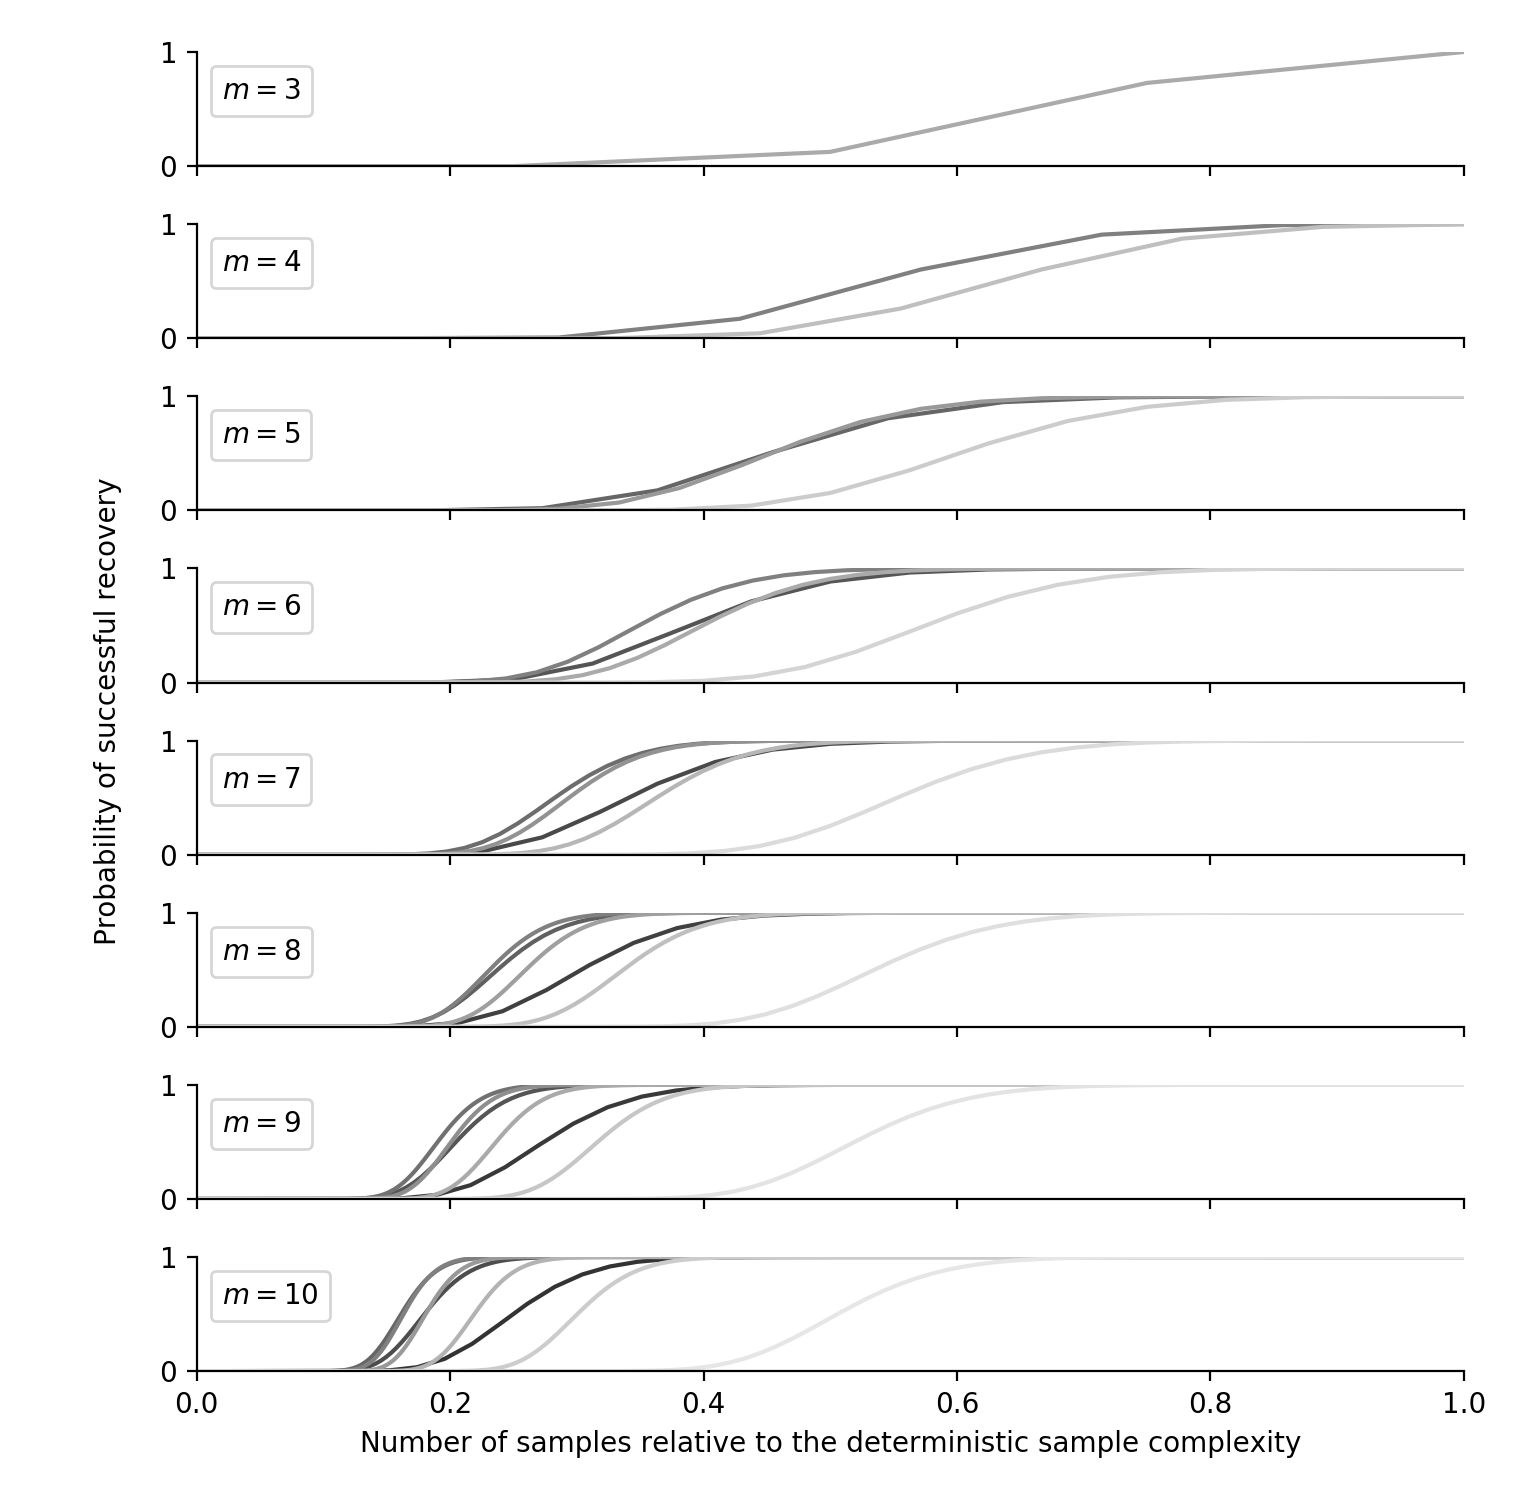
\includegraphics[width=1 \linewidth]{figures/prob_vs_samples.png}
\caption{\textbf{Learning a dictionary from an arbitrary number of samples.} Probability of successful dictionary and code recovery (as per Thm. \ref{DeterministicUniquenessTheorem}) for a number of samples $N$ given as a fraction of the deterministic sample complexity $N = |\mathcal{H}|[(k-1){m \choose k} + 1]$ when the support set hypergraph $\mathcal{H}$ is the set of $m$ consecutive intervals of length $k$ in a cyclic order on $[m]$. Each plot has $k$ ranging from $2$ to $m-1$ (the case $k=1$ requires $N=m$), with lighter grey lines corresponding to larger $k$. Successful recovery is nearly certain with far fewer samples than the deterministic sample complexity. }
\vspace{-.6 cm}
\label{probvsamples}
\end{center}
\end{figure}

\begin{figure}\label{reasonableC2}
\begin{center}
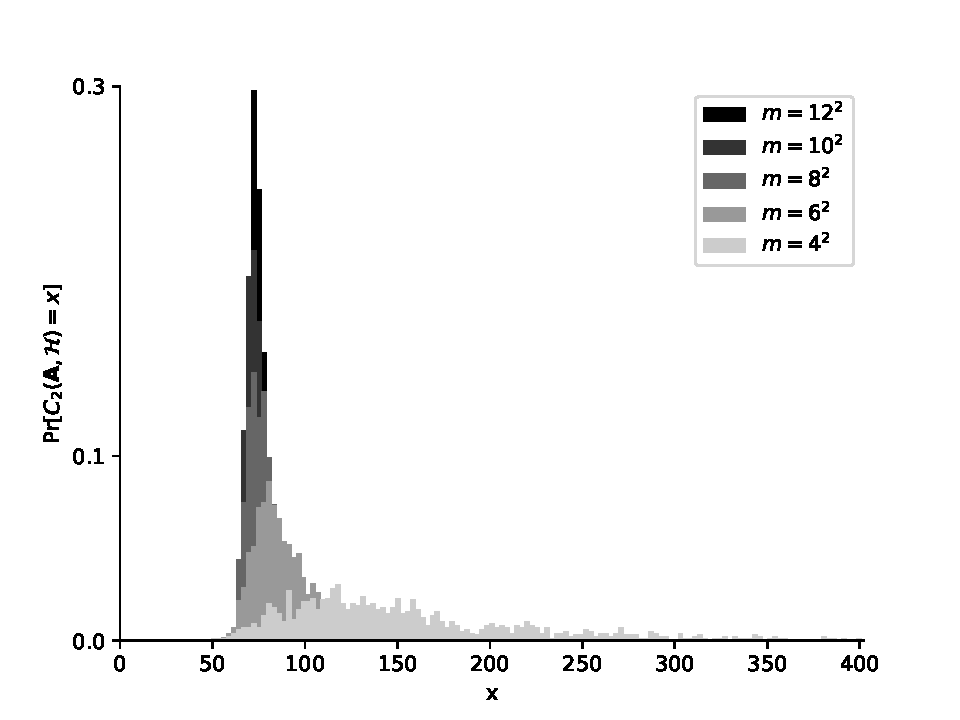
\includegraphics[width=1 \linewidth]{figures/C2.pdf}
\caption{\textbf{Concentration of the constant $C_2$.} Distribution of $C_2(\mathbf{A}, \mathcal{H})$ computed for 1.33x overcomplete generic unit-norm dictionaries $\mathbf{A} \in \mathbb{R}^{n \times m}$ (i.e. with $n = 3m/4$) when the support set hypergraph $\mathcal{H}$ consists of the rows and columns formed by arranging  the elements of $[m]$ into a square grid (i.e. $m = k^2$). The distribution becomes more concentrated as $m$ grows.}
\vspace{-.6 cm}
\label{samples_vs_m}
\end{center}
\end{figure}


